\documentclass[fleqn,10pt]{wlscirep}
\usepackage[utf8]{inputenc}
\usepackage[T1]{fontenc}
\usepackage{siunitx}
\usepackage{placeins}
\graphicspath{{figures/}}
\title{BioInteract: Interpretable Drug--Target Interaction Prediction via
  Residue-Level Cross-Attention with Biological Prior Knowledge}

\author[1,+]{Shengnan Wang}
\author[2,+]{Qi Zhang}
\author[2]{Xucheng Liu}
\author[2]{Zixuan Wang}
\author[2]{Jiangke Cheng}
\author[3,4]{Zhi Huang*}
\affil[1]{School of Biological and Chemical Engineering,
  Panzhihua University, Panzhihua 617000, P.R.\ China}
\affil[2]{School of Mathematics and Computer Science,
  Panzhihua University, Panzhihua 617000, P.R.\ China}
\affil[3]{Department of Environmental Science and Engineering,
  College of Architecture and Environment,
  Sichuan University, Chengdu 610065, P.R.\ China}
\affil[4]{Institute of New Energy and Low Carbon Technology,
  Sichuan University, Chengdu 610065, P.R.\ China}

\affil[*]{corresponding.author. E-mail: 525514353@qq.com}

\affil[+]{these authors contributed equally to this work}

% \keywords{Drug--target interaction; interpretable deep learning; cross-attention; graph
% neural network; protein language model; binding site prediction}

\begin{abstract}
Accurate prediction of drug--target interactions (DTIs) can support the prioritisation of candidate pairs, yet many deep-learning models provide little visibility into the features used for prediction. We present BioInteract, a DTI framework combining a chemistry-aware molecular graph encoder, an ESM-2/physicochemical protein residue encoder with a configured domain-label channel, and bidirectional cross-attention. The model produces atom--residue attention matrices and atom-level Grad-CAM scores as model-native attribution outputs. A full-precision reconstruction from the released random-split checkpoint and inputs achieved an AUROC of 0.904 on the Davis kinase inhibitor benchmark; the corresponding entity-held-out reconstructions are reported with their complete provenance. We additionally audit chemical and sequence similarity across these partitions and evaluate exact-sequence-grouped cold-start protocols. On a strict exact-entity-novel BindingDB cohort, the frozen Davis checkpoint achieved an AUROC of 0.560 and an AUPRC of 0.340, indicating limited external transfer. The attribution analyses generate hypotheses about model-relevant atoms and residues, but do not constitute predicted three-dimensional contacts or structural mechanisms. The released input package contains no curated per-protein domain annotations, so the domain-label channel uses its unknown label and is not treated as domain evidence. BioInteract therefore provides a transparent starting point for prioritisation and for experimentally testable hypotheses, subject to the dataset and structural-validation limitations stated below.
\end{abstract}
\begin{document}

\flushbottom
\maketitle
% * <john.hammersley@gmail.com> 2015-02-09T12:07:31.197Z:
%
%  Click the title above to edit the author information and abstract
%
\thispagestyle{empty}
\section*{Keywords}

Drug--target interaction; interpretable deep learning; cross-attention; graph
neural network; protein language model; model attribution
%%====================================================================
\section{Introduction}
\label{sec:introduction}
%%====================================================================

The emergence of ``AI for Science'' has increased expectations that
computational models should not merely maximise predictive accuracy, but should
also expose the evidence and uncertainty needed for scientific hypothesis
generation.\cite{schneider2020rethinking}  This expectation is especially
important in drug discovery, where identifying drug--target interactions (DTIs)
requires reliable prioritisation together with inspectable outputs that can
guide, but not replace, mechanistic follow-up.

Experimental profiling of binding affinities through surface plasmon resonance,
isothermal titration calorimetry, or kinase activity assays is laborious and
prohibitively expensive.  The Davis kinase inhibitor
dataset\cite{davis2011comprehensive} alone required systematic measurement
of 72 inhibitors against 442 kinases---a campaign spanning only a fraction of
the druggable proteome.  Computational DTI prediction can ease this bottleneck
by prioritising the most promising candidates and thereby reducing cost and
attrition in development
pipelines.\cite{chen2016drug,yamanishi2008prediction}  Yet the field has
largely remained trapped in a \emph{predictive-accuracy race}: successive deep
learning architectures---DeepDTA,\cite{ozturk2018deepdta}
GraphDTA,\cite{nguyen2021graphdta}
MolTrans,\cite{huang2021moltrans}
DrugBAN\cite{bai2023drugban}---have incrementally improved benchmark metrics
while leaving an important modelling question only partly addressed:
\emph{which input features drive a given prediction?}

This question lies at the heart of the broader ``AI for Science'' agenda.  A
prediction with no interpretable output is, at best, a hypothesis generator.
Moving from \emph{prediction} to hypothesis generation therefore benefits from
models that expose internal attribution patterns---for example, attention
distributed across drug atoms and protein residues and gradient-based atom
scores---rather than returning only a scalar probability.  These outputs can
prioritise follow-up experiments, but they are not direct measurements of
physical contacts or pocket geometry.

Classical DTI methods illuminate the fundamental tension between interpretability
and accuracy.  Structure-based approaches (molecular docking, molecular dynamics)
provide structural inference anchored in three-dimensional protein
geometry,\cite{kitchen2004docking} yet are constrained by the availability of
high-quality crystal structures and the steep computational cost of free-energy
calculations.  Ligand-based methods (QSAR, molecular
fingerprints)\cite{cherkasov2014qsar} circumvent structural requirements at
the expense of mechanistic transparency.  Neither paradigm fully satisfies the
twin demands of modern drug discovery.

Deep learning has transformed predictive capabilities in this domain.
Pretrained protein language models such as ESM-2\cite{lin2023evolutionary}
encode evolutionary and structural information at residue resolution, while
graph neural networks faithfully capture molecular topology.  Concurrently,
chemical language models have demonstrated that pretrained molecular
representations support accurate and interpretable prediction of reactivity and
toxicity,\cite{huang2025large} and chemistry-enhanced transformer
architectures such as Radical-Net recover atom-level reaction
mechanisms.\cite{huang2025radical}  Together, these advances underscore
the importance of domain-specific pretraining and chemistry-aware inductive
biases in molecular AI;\cite{huang2024ai} their integration into
interpretable DTI frameworks, however, has remained limited.

In this study, ``biological prior knowledge'' refers specifically to the
sequence information encoded by frozen ESM-2 pretraining together with explicit
per-residue physicochemical descriptors. It does not denote curated Pfam,
InterPro, binding-site, or other protein-domain annotations.

The ``AI for Science'' paradigm benefits from attribution mechanisms that are
part of the prediction pathway rather than appended only after training.
Attention visualisation and SHapley Additive exPlanations (SHAP) can nevertheless
have faithfulness limitations.\cite{jain2019attention} A central principle is
therefore that, when attention is an integral component of the prediction
pathway, the resulting attributions can be examined consistently with model
output but still require external validation before mechanistic interpretation.

Motivated by these observations, we present \textbf{BioInteract}, a framework
that brings model-native attribution outputs to binary high-affinity DTI
classification.  BioInteract rests on three architectural components:

\begin{enumerate}[leftmargin=*]
\item \textbf{Chemistry-aware molecular graph encoding.}  Drug molecules are
  represented as attributed graphs encoding functional-group-relevant properties
  (H-bond donor/acceptor status, hydrophobicity, partial charges) that
  are available to the learned molecular representation.

\item \textbf{Protein residue encoding with a disclosed domain-label limit.}
  Protein representations fuse ESM-2 residue embeddings with per-residue
  physicochemical properties and a configured domain-label channel. No curated
  per-protein domain-annotation files are present in the released Davis input
  package; the channel therefore receives the unknown label at every position
  and is not interpreted as Pfam/InterPro information.

\item \textbf{Bidirectional cross-attention attribution module.}  A multi-head
  cross-attention mechanism computes a matrix
  $\mathbf{M} \in \mathbb{R}^{n_\text{atoms} \times n_\text{residues}}$ of
  learned attention weights between drug-atom and protein-residue
  representations.  The matrix is an integral component of the forward pass;
  it is used here as a model-native attribution output, not as a predicted
  atom-level structural contact map.
\end{enumerate}

We evaluate BioInteract on the Davis kinase inhibitor
dataset\cite{davis2011comprehensive} under a random pair split and two
entity-held-out protocols: Drug-ID-held-out and Target-ID-held-out. We report
chemical and sequence-similarity
diagnostics for these partitions, because identifier-level exclusion alone does
not guarantee scaffold- or sequence-level novelty.  We also add
exact-sequence-grouped cold-target and exact-sequence-grouped cold-both
evaluations.  The attribution
analyses---cross-attention maps, Grad-CAM scores, attention-concentration
summaries, and case studies---are interpreted as model behaviour rather than as
independent evidence of molecular recognition mechanisms.

%%====================================================================
\section{Related Work}
\label{sec:related}
%%====================================================================

\subsection{Deep Learning for DTI Prediction}

Deep learning approaches to DTI prediction have evolved through several
generations.\cite{wen2017deep}  \emph{Sequence-based} models encode both
drug SMILES and protein amino acid sequences as one-dimensional strings.
DeepDTA\cite{ozturk2018deepdta} employs parallel one-dimensional convolutional
neural networks (CNNs) for drug and
protein encoding; WideDTA\cite{ozturk2019widedta} extends this framework
with additional molecular descriptors.  Although computationally efficient, these
models discard molecular topology and are limited in their capacity to model
long-range intramolecular interactions.

\emph{Graph-based} models overcome this limitation by representing drugs as
attributed molecular graphs.  GraphDTA\cite{nguyen2021graphdta} benchmarks a
graph convolutional network (GCN), graph attention network (GAT), graph
isomorphism network (GIN), and hybrid GAT--GCN encoder while retaining a CNN
for proteins.  MolTrans\cite{huang2021moltrans} introduces mutual
interaction learning between molecular substructure representations and protein
subsequences.

\emph{Attention-based} models include architectures that learn local or
cross-modal representations for DTI/DTA prediction.
TransformerCPI\cite{chen2020transformercpi} applies transformer attention to
drug--protein interaction patterns.  DrugBAN\cite{bai2023drugban} introduces
a dual bilinear attention network for fine-grained local interaction modelling.
AttentionDTA\cite{zhao2022attentiondta} employs multi-head self-attention for
both drug and protein representations.  In most prior work, however, attention
operates as a computational device rather than as an interpretable output channel.

\subsection{Pretrained Protein Language Models}

ESM-2,\cite{lin2023evolutionary} trained on millions of protein sequences
via masked language modelling, produces residue-level embeddings that encode
evolutionary conservation, secondary structure propensity, and contact
information.  These pretrained representations substantially outperform
hand-crafted features on downstream tasks.\cite{rives2021biological}  In DTI
prediction, pretrained representations have already been combined with graph
drug encoders and interaction modules.  For example, GEFA uses pretrained
protein representations in an early-fusion graph architecture,\cite{nguyen2022gefa}
PGraphDTA replaces a CNN target encoder with protein language-model features,
\cite{bal2023pgraphdta} and HCAF-DTA combines protein representations with
bidirectional cross-attention.\cite{li2025hcafdta}  BioInteract therefore does
not claim to be the first application of a protein language model, a graph
encoder, or cross-attention to DTI/DTA prediction.  Its specific contribution is
the submitted integration of a chemistry-aware molecular graph encoder,
residue-level ESM-2/physicochemical features with a configured domain-label
channel, and inspectable model-native attribution
outputs for the Davis binary-classification setting.  These outputs are not
treated as biologically grounded structural evidence without independent
validation.

Recent DTA studies also illustrate the use of residue-level protein graphs,
domain-specific representations, or biological-context features alongside
evaluation on more than one benchmark, including 3DProtDTA,\cite{voitsitskyi2023_3dprotdta}
the domain-specific framework of Liu \textit{et al.},\cite{liu2024domainspecific}
and InceptionDTA.\cite{kalemati2025inceptiondta}  We cite these studies to
contextualise the requested external evaluation, rather than treating their
reported results as directly comparable baselines under the present Davis binary
classification protocol.

\subsection{Interpretability in DTI Models}

Existing interpretability approaches include post-hoc methods (attention-weight
visualisation, gradient-based attribution, and SHAP values\cite{jimenez2020drug})
and model-native attribution mechanisms.  Attention weights do not necessarily
equal feature importance.\cite{jain2019attention}  BioInteract uses a
cross-attention matrix that contributes to prediction and can be inspected as a
model-native attribution.  It does not by itself establish atom-level contacts,
binding modes, or physical interaction types.  In contrast, models such as
MONN use explicit non-covalent interaction supervision derived from structural
complexes;\cite{li2020monn} no comparable supervision is used here.

\subsection{Cold-Start Evaluation}

Random-split evaluation permits information leakage through shared drugs or
targets between training and test sets, yielding inflated
estimates.\cite{huang2021therapeutics}  Cold-start protocols address this by
ensuring that test identifiers are absent from training data. We report the
original Drug-ID-held-out and Target-ID-held-out protocols alongside the random
split, and separately use exact-sequence grouping for stricter within-Davis
stress tests.

%%====================================================================
\section{Methods}
\label{sec:methods}
%%====================================================================

\subsection{Problem Formulation}

Given a drug molecule $d$ represented by its SMILES string and a target protein
$t$ represented by its amino acid sequence, we formulate DTI prediction as
binary classification: predict whether $d$ binds $t$ with high affinity.
Following the established protocol for the Davis
dataset,\cite{davis2011comprehensive} continuous $K_d$ values are binarised
at \SI{30}{nM} ($pK_d > 7.52$), classifying pairs with $K_d < \SI{30}{nM}$ as
positive interactions.

\subsection{Architecture Overview}

BioInteract comprises five sequential modules:
(1)~a graph isomorphism network with edge features (GINE)-based drug encoder producing per-atom representations,
(2)~a target encoder combining ESM-2 embeddings with physicochemical features
and a configured domain-label channel,
(3)~a bidirectional cross-attention module computing attention matrices between
ligand-atom and protein-residue representations,
(4)~gated attention pooling to aggregate variable-length representations, and
(5)~a multilayer perceptron (MLP) prediction head.
The full model contains 2{,}442{,}083 trainable parameters.

\subsection{Drug Molecular Graph Encoder}

\subsubsection{Chemistry-Aware Atom Featurisation}

Each atom is represented by a 52-dimensional feature vector encoding:
\begin{itemize}[leftmargin=*]
\item \textbf{Topological features} (38 dimensions): atom type (one-hot,
  20 types), hybridisation state (6), formal charge (6), number of
  attached hydrogens (6).
\item \textbf{Structural features} (9 dimensions): degree, aromaticity, ring
  membership, and ring size membership (3--8).
\item \textbf{Functional features} (5 dimensions): hydrogen-bond donor and
  acceptor status, Crippen logP contribution, molar refractivity, and Gasteiger
  partial charge.
\end{itemize}
Bond features (16 dimensions) encode bond type, conjugation, ring membership,
and stereochemistry.

\subsubsection{GINE Message Passing}

We employ a 3-layer GINE
architecture:\cite{hu2020strategies}
\begin{equation}
\widetilde{\mathbf{e}}_{vu}=\mathbf{W}_e\mathbf{e}_{vu}+\mathbf{b}_e
\in\mathbb{R}^{256},\qquad \mathbf{e}_{vu}\in\mathbb{R}^{16},
\label{eq:edge_projection}
\end{equation}
\begin{equation}
\mathbf{h}_v^{(\ell+1)} = \mathrm{MLP}^{(\ell)}\!\left(
  \mathbf{h}_v^{(\ell)} +
  \sum_{u\in\mathcal{N}(v)}
  \mathrm{ReLU}\!\left(\mathbf{h}_u^{(\ell)} + \widetilde{\mathbf{e}}_{vu}\right)
\right)
\end{equation}
where $\mathbf{h}_v^{(\ell)}$ is the representation of atom $v$ at layer $\ell$,
$\mathbf{e}_{vu}$ denotes the raw 16-dimensional edge feature vector, and
$\widetilde{\mathbf{e}}_{vu}$ is its learned 16-to-256 projection before message
passing. The released \texttt{GINEConv} instantiation uses the default fixed
$\epsilon=0$. Each layer incorporates batch normalisation, ReLU activation,
dropout ($p=0.2$), and a residual connection; the hidden dimension is $D=256$.
Global graph pooling is \emph{not} applied at this stage, preserving individual
atom representations for the subsequent cross-attention step.

The archived checkpoints use the stated molecular featurisation; public
checkpoint reconstruction applies no stochastic graph augmentation.

\subsection{Protein Target Encoder}

\subsubsection{ESM-2 Residue Embeddings}

Residue-level representations are extracted from ESM-2 (150\,M parameters,
\texttt{esm2\_t30\_150M\_UR50D}),\cite{lin2023evolutionary} yielding
640-dimensional embeddings for each amino acid.  These embeddings encode
evolutionary conservation, secondary structure propensity, and long-range contact
information learned from 65 million protein sequences.  ESM-2 parameters are
frozen throughout training.

\subsubsection{Physicochemical Property Encoding}

Each residue is augmented with a 4-dimensional physicochemical vector:
\begin{equation}
\mathbf{p}_i = \bigl[\text{hydrophobicity}_i,\;\text{mol.\ weight}_i,\;
  \text{charge}_i,\;\text{polarity}_i\bigr]
\end{equation}
Hydrophobicity follows the Kyte--Doolittle scale.\cite{kyte1982simple}
These values provide residue-level physicochemical descriptors; by themselves,
they do not identify pocket membership, solvent exposure, or interaction
partners.

\subsubsection{Configured Domain-Label Channel and Availability}

The implementation contains a learnable domain-label embedding layer:
\begin{equation}
\mathbf{d}_i = \mathrm{DomainEmbed}(\text{domain\_type}_i) \in \mathbb{R}^{32}
\end{equation}
The label builder assigns the unknown \texttt{NONE} type when a per-protein
annotation file is unavailable. The released Davis package contains no such
annotation files, so all archived input positions use this unknown label. We
therefore do not represent this channel as curated Pfam/InterPro context, as a
binding-site label, or as evidence for a domain-specific conclusion.

\subsubsection{Feature Fusion}

The three feature sources are concatenated and projected through a shared linear
transformation:
\begin{equation}
\mathbf{r}_i = \mathrm{Proj}\!\left(
  [\mathbf{e}_i \,\|\, \mathbf{p}_i \,\|\, \mathbf{d}_i]
\right) \in \mathbb{R}^{D}
\end{equation}
where $\mathbf{e}_i \in \mathbb{R}^{640}$ is the ESM-2 embedding and Proj is a
two-layer MLP with layer normalisation and Gaussian error linear unit (GELU)
activation. In the released configuration, $\mathbf{d}_i$ is the shared unknown
domain-label embedding rather than a curated per-residue annotation. The projected
dimension $D=256$ matches the drug encoder output.

\subsection{Cross-Attention Interaction Module}

The cross-attention module produces the model-native attribution used in this
study. It computes bidirectional attention between ligand-atom and
protein-residue representations, producing an explicit atom--residue attention
matrix.

\subsubsection{Drug-to-Protein Attention}

\begin{equation}
\mathrm{Attn}(\mathbf{Q}_d,\mathbf{K}_p,\mathbf{V}_p) =
  \mathrm{softmax}\!\left(\frac{\mathbf{Q}_d\mathbf{K}_p^\top}{\sqrt{d_k}}\right)
  \mathbf{V}_p
\end{equation}
where $\mathbf{Q}_d = \mathbf{H}_d\mathbf{W}_Q^d$,
$\mathbf{K}_p = \mathbf{R}\mathbf{W}_K^p$,
$\mathbf{V}_p = \mathbf{R}\mathbf{W}_V^p$, with $H=8$ heads and head
dimension $d_k = D/H = 32$.

\subsubsection{Protein-to-Drug Attention}

Symmetrically, protein residues attend over drug atoms:
\begin{equation}
\mathrm{Attn}(\mathbf{Q}_p,\mathbf{K}_d,\mathbf{V}_d) =
  \mathrm{softmax}\!\left(\frac{\mathbf{Q}_p\mathbf{K}_d^\top}{\sqrt{d_k}}\right)
  \mathbf{V}_d
\end{equation}

\subsubsection{Attribution Map Extraction}

The atom--residue attribution map is obtained by averaging drug-to-protein
attention weights across all heads:
\begin{equation}
\mathbf{M} = \frac{1}{H}\sum_{h=1}^{H}
  \mathrm{Attn}_h(\mathbf{Q}_d,\mathbf{K}_p)
  \;\in\;\mathbb{R}^{n\times L}
\label{eq:interaction_map}
\end{equation}
Because $\mathbf{M}$ is computed within the forward pass rather than post-hoc,
it is a model-native attribution matrix.  It is not interpreted as a physical
contact map or as an assignment of a specific interaction type to an atom pair.

\subsection{Gated Pooling and Prediction}

Variable-length representations are aggregated via gated attention pooling:
\begin{equation}
\mathbf{z} = \sum_{i}\alpha_i\cdot g(\mathbf{x}_i),\qquad
\alpha_i = \frac{\exp(f(\mathbf{x}_i))}{\sum_j\exp(f(\mathbf{x}_j))}
\end{equation}
where $f\colon\mathbb{R}^D\to\mathbb{R}$ and
$g\colon\mathbb{R}^D\to\mathbb{R}^D$ are learned two-layer MLPs with Tanh
activation.  The pooled drug and protein representations are concatenated and
passed through a two-hidden-layer MLP (256\,$\to$\,128; ReLU; dropout $p=0.3$)
followed by sigmoid activation to produce the binding probability.

\subsection{Training Provenance and Evaluation Thresholds}

The archived entity-split checkpoints preserve model architecture but do not
store a uniform optimizer, scheduler, warmup, or label-smoothing record. The
Random and Drug-ID-held-out logs explicitly record weighted binary
cross-entropy, label smoothing of 0.05, AdamW, and a final-run header, whereas
the checkpoint-matched Target-ID-held-out trace has the older
\texttt{run\_split.py} header and records only loss and validation AUROC. Its
checkpoint does not retain optimizer or loss state. We therefore do not
retrospectively assert a single training recipe across all three historical
checkpoints (Supporting Information, Training-provenance table).

No historical entity-split model is retrained for the current-release metrics.
The canonical reconstruction instantiates each of those three released
checkpoints from its embedded model configuration, performs full-precision
inference, selects an F1 threshold once on the corresponding validation
predictions, and applies that frozen threshold to test predictions. This
separation prevents test-set threshold selection.

In contrast, the two exact-sequence-grouped strict protocols were trained from
initialisation on their respective new training partitions. They use seed 42,
the same Davis preprocessing and architecture, weighted binary cross-entropy
with 0.05 label smoothing, AdamW (learning rate $10^{-4}$; weight decay
$10^{-5}$), batch size 64, gradient-norm clipping at 1.0, a five-epoch linear
warm-up followed by cosine decay, and a maximum of 100 epochs. The checkpoint
with the highest validation AUROC was selected with patience 15, after which an
F1 threshold was selected on that protocol's validation predictions and frozen
for its test evaluation. Complete strict-split training provenance, checkpoint
paths, SHA-256 hashes, selected epochs, and thresholds are provided in the
Supporting Information Training-provenance table.

\subsection{Interpretability Analysis}

\subsubsection{Residue-Level Attention Profiling}

For a given drug--target pair, per-residue attention scores are obtained by
summing the interaction map over all drug atoms:
\begin{equation}
s_j = \sum_{i=1}^{n} M_{ij},\quad j=1,\ldots,L
\end{equation}
These values are model-attribution scores and are not assigned a biological
hotspot label.

\subsubsection{Grad-CAM Functional-Group Attribution}

Grad-CAM\cite{selvaraju2017grad} is adapted to the graph-neural-network (GNN)
setting:
\begin{equation}
\mathrm{CAM}_v = \mathrm{ReLU}\!\left(\sum_k w_k\cdot A_v^k\right),\quad
w_k = \frac{1}{|\mathcal{V}|}\sum_v\frac{\partial z}{\partial A_v^k}
\end{equation}
where $A_v^k$ is channel $k$ of the third (final) GINE message-passing layer
and $z$ is the pre-sigmoid positive-class logit. Gradients are therefore taken
with respect to the logit, not the post-sigmoid probability.
Functional groups are detected with predefined SMARTS patterns (aromatic ring,
hydroxyl, amino, amide, carboxyl, sulfonyl, halogen, ether, heterocycle N, and
carbonyl). For each group, all RDKit substructure matches are merged into a
deduplicated atom set and the group score is the mean of the normalised
atom-level scores over that set. An atom can match more than one group pattern.
These scores indicate sensitivity of the prediction to the learned
representation and do not identify chemical bonds or contacts in a
three-dimensional complex.

\subsubsection{Attention Sparsity}

For each drug--target pair, residue scores are normalised by that pair's maximum:
\begin{equation}
\widetilde{s}_j = \frac{s_j}{\max_k s_k}.
\end{equation}
Pair-level sparsity is then
\begin{equation}
\mathrm{Sparsity} = \frac{|\{j : \widetilde{s}_j < 0.1\}|}{L}.
\end{equation}
The reported global value uses all 1{,}506 positive Davis records, rather than a
single test partition, evaluated with the archived \texttt{checkpoints/best.pt}
checkpoint. Each pair is normalised separately; the 1{,}301{,}380 valid-residue
scores are then concatenated before the global distribution and fraction are
computed. Consequently, all original train/validation/test memberships are
represented and longer valid target sequences contribute more residue-level
observations.

%%====================================================================
\section{Experimental Setup}
\label{sec:experiments}
%%====================================================================

\subsection{Dataset}

The Davis kinase inhibitor
dataset\cite{davis2011comprehensive} comprises 68 drugs (kinase inhibitors)
and 442 targets (protein kinases) forming 30{,}056 drug--target pairs.  Binding
affinities ($K_d$) are binarised at \SI{30}{nM}, yielding approximately
\SI{5}{\percent} positive interactions.

\subsection{Pre-specified External BindingDB Evaluation}

To test exact-entity transfer without changing the submitted Davis training
protocol, we curated the official BindingDB curated-articles snapshot
\texttt{BindingDB\_BindingDB\_Articles\_202607}\cite{gilson2016bindingdb}.
We retained only finite, exact numerical $K_d$ measurements in nM for valid,
single-chain proteins of at most 1{,}200 residues and RDKit-valid ligands.
Inequality-qualified values were excluded. Before replicate reconciliation, any
external pair was excluded when its canonical isomeric
SMILES occurred anywhere in Davis or when its full normalised amino-acid
sequence occurred anywhere in Davis.  The resulting cohort is therefore
double-novel by exact ligand and target-sequence identity, although it is not a
claim of scaffold or remote-homology novelty. Measurements were then grouped by
canonical ligand--sequence pair. A pair with replicate measurements on opposite
sides of the \SI{30}{nM} boundary was removed (a pair-level conflict); for every
remaining pair, the median exact $K_d$ was retained and binarised as
$K_d<\SI{30}{nM}$. The complete row-to-pair accounting is reported in
Table~S13.

The released \texttt{best\_random} checkpoint was evaluated without retraining,
fine-tuning, calibration, or threshold selection on BindingDB.  We used the
existing random-validation threshold of 0.5959881544 and the same
640-dimensional ESM-2 representation used for Davis. Only newly extracted
external protein embeddings that passed dimension and sequence-length checks
were supplied to the frozen model.
AUROC and AUPRC confidence intervals use 600 pair-stratified bootstrap
replicates with seed 42.  Curation and frozen-inference provenance, including
source and prediction hashes, are reported in Table~S13.

\subsection{Data Splitting Protocols and Similarity Audit}

\begin{itemize}[leftmargin=*]
\item \textbf{Random split} (70/10/20): drug--target pairs are assigned randomly;
  shared entities may appear across splits.
\item \textbf{Drug-ID-held-out split}: drugs are partitioned such that all interactions
  of a given compound identifier appear in exactly one split.  This prevents
  drug-identifier overlap but does not impose a scaffold-similarity threshold.
\item \textbf{Target-ID-held-out split}: targets are partitioned analogously; test
  target identifiers are absent from training.  This initial entity-held-out
  protocol does not impose a sequence-similarity threshold.
\end{itemize}

For the Drug-ID-held-out audit, we computed non-chiral radius-2, 1024-bit Morgan
fingerprints with RDKit and
reported the maximum Tanimoto similarity between each test compound and the
training compounds. For the Target-ID-held-out audit, we used RapidFuzz
\texttt{fuzz.ratio}, divided by 100, where normalised Indel similarity is
$1-d_\mathrm{Indel}/(|x|+|y|)$ and substitutions are represented by one
deletion plus one insertion. We computed the maximum value between each test
sequence and all training sequences and separately identified exact duplicate
sequences. The original
Target-ID-held-out partition contained six exact-sequence groups crossing the
training and test sets. We additionally constructed exact-sequence-grouped cold-target
and exact-sequence-grouped cold-both partitions, assigning all target identifiers with an identical
amino-acid sequence to the same split.  These reviewer-requested protocols use
the same Davis records, 70/10/20 partition ratios, and seed 42.

For the strict cold-both protocol, the 70/10/20 ratios are applied independently
to drug identifiers and exact target-sequence groups. Only pairs for which both
entities belong to the same train, validation, or test block are retained;
cross-block combinations are excluded to prevent either entity from crossing a
partition. Consequently, the retained pair counts are 15{,}190/264/1{,}144,
and the pair-level proportions are not 70/10/20. Of the 30{,}056 Davis pairs,
13{,}458 cross-block pairs are not used in this cold-both evaluation.

To quantify residual target relatedness after exact-sequence grouping, we used
Biopython \texttt{Align.PairwiseAligner} in global mode (match $=1$, mismatch
$=0$, gap opening $=-1$, gap extension $=-0.5$) to align each
exact-sequence-grouped cold-target
test sequence against every training sequence. Identity is the number of
exact-residue matches divided by full alignment length; the maximum is retained
for each test target. We also implemented leakage-aware diagnostic controls on
this same exact-sequence-grouped cold-target partition. A drug-only control uses non-chiral
radius-2, 1024-bit
Morgan fingerprints in a logistic-regression classifier; a drug-promiscuity
control uses each drug's positive prevalence estimated only from training
targets; and a label-shuffled drug-only control permutes training labels while
leaving test labels unchanged.  Because every target identifier in this split
is unseen, a target-specific degree computed from its full label column would
leak test labels; the only target-only control that avoids that leakage assigns
the training positive prevalence uniformly.  These controls are diagnostic
rather than capacity-matched replacements for BioInteract.

\subsection{Evaluation Metrics}

For binary classification under severe class imbalance, we report AUROC and
AUPRC as primary metrics---AUPRC is particularly informative because it measures
positive-class precision across all recall levels. For every reported protocol,
F1, precision, and recall use a decision threshold selected once on the
corresponding validation precision--recall curve; AUROC and AUPRC remain
threshold-free.

\subsection{Implementation}

BioInteract is implemented in Python~3.10.14 using PyTorch~2.4.0+cu121 and
PyTorch Geometric~2.6.1.\cite{fey2019fast} Protein embeddings are extracted using
ESM-2\cite{lin2023evolutionary} (\texttt{esm2\_t30\_150M\_UR50D}, 640
dimensions; \texttt{fair-esm}~2.0.0). Molecular featurisation is performed with
RDKit~2025.03.6.\cite{rdkit} Revision diagnostics additionally use
Biopython~1.87 and RapidFuzz~3.14.5. Training employs automatic mixed precision (AMP) for
memory efficiency on a single NVIDIA GPU. Final checkpoint evaluation is run
under \texttt{torch.inference\_mode()} in full precision, using each checkpoint's
embedded architecture configuration.

%%====================================================================
\section{Results}
\label{sec:results}
%%====================================================================

\subsection{Comparison with Baseline Methods}

We compare BioInteract against six published DTI baselines spanning
sequence, graph, attention, transformer, and bilinear interaction models:
DeepDTA,\cite{ozturk2018deepdta} GraphDTA,\cite{nguyen2021graphdta}
AttentionDTA,\cite{zhao2022attentiondta} MolTrans,\cite{huang2021moltrans}
TransformerCPI,\cite{chen2020transformercpi} and DrugBAN.\cite{bai2023drugban}
The methods span sequence CNNs, molecular graphs, self-attention,
transformer interaction models, and bilinear attention (Table~\ref{tab:comparison}).

\begin{table}[htbp]
\centering
\caption{Comparison of BioInteract with baseline methods on the Davis dataset
  under three identifier-based splitting protocols (binary classification,
  $K_d < \SI{30}{nM}$). Best value in each column is in \textbf{bold}.}
\label{tab:comparison}
\resizebox{\textwidth}{!}{%
\begin{tabular}{@{}llcccccc@{}}
\toprule
 & & \multicolumn{2}{c}{\textbf{Random}} &
     \multicolumn{2}{c}{\textbf{Target-ID-held-out}} &
     \multicolumn{2}{c}{\textbf{Drug-ID-held-out}} \\
\cmidrule(lr){3-4}\cmidrule(lr){5-6}\cmidrule(lr){7-8}
\textbf{Method} & \textbf{Paradigm} & AUROC & AUPRC & AUROC & AUPRC & AUROC & AUPRC \\
\midrule
DeepDTA\cite{ozturk2018deepdta}             & Seq-CNN     & 0.878 & 0.352 & 0.783 & 0.247 & 0.592 & 0.089 \\
GraphDTA\cite{nguyen2021graphdta}           & GNN+CNN     & 0.893 & 0.403 & 0.815 & 0.312 & 0.621 & 0.102 \\
AttentionDTA\cite{zhao2022attentiondta}     & Self-Attn   & 0.900 & 0.425 & 0.838 & 0.348 & 0.643 & 0.108 \\
MolTrans\cite{huang2021moltrans}            & Transformer & 0.907 & 0.480 & 0.856 & 0.389 & 0.668 & 0.121 \\
TransformerCPI\cite{chen2020transformercpi} & Transformer & 0.910 & 0.492 & 0.862 & 0.401 & 0.672 & 0.125 \\
DrugBAN\cite{bai2023drugban}                & Bilinear    & \textbf{0.915} & 0.530 & 0.874 & 0.428 & 0.695 & 0.138 \\
\midrule
\textbf{BioInteract (Ours)} & Cross-Attn & 0.904 & \textbf{0.560} & \textbf{0.930} & \textbf{0.525} & \textbf{0.733} & \textbf{0.167} \\
\bottomrule
\end{tabular}
}
\end{table}

\begin{figure}[htbp]
\centering

\includegraphics[width=\textwidth]{figures/fig_comparison_random.pdf}\par\vspace{8pt}

\includegraphics[width=0.78\textwidth]{figures/fig_comparison_splits.pdf}
\caption{\textbf{Baseline comparison.} Panels A and B show random-split AUROC
  and AUPRC, respectively, for all methods. Panel C shows AUROC under the
  random, Target-ID-held-out, and Drug-ID-held-out protocols. BioInteract
  attains the highest random-split AUPRC and the highest AUROC and AUPRC in the
  two identifier-held-out protocols.}
\label{fig:comparison}
\end{figure}

\FloatBarrier

On the random split, BioInteract has the highest AUPRC (0.560), while DrugBAN
has the highest AUROC (0.915). BioInteract attains the highest AUROC and AUPRC
under the Target-ID-held-out and Drug-ID-held-out protocols. Because the
baselines do not use a matched protein-pretraining regime, these comparisons
provide benchmark context rather than a controlled attribution of performance
to a single architectural component.

Under the Drug-ID-held-out protocol, BioInteract obtained AUROC~$=0.733$ in the
current-release reconstruction. The maximum test-to-training Morgan Tanimoto similarity
ranged from 0.196 to 0.538 (median 0.257), documenting identifier-level
compound exclusion while also making the remaining chemical-neighbourhood
relation explicit.

\subsection{Ablation Study}

We assessed the contribution of the principal architectural components by
removing one component at a time from the full model (Table~\ref{tab:ablation}
and Fig.~\ref{fig:ablation}).

\begin{table}[htbp]
\centering
\caption{Ablation study on the Davis dataset. Each row reports the full model or
  a variant with one component removed.}
\label{tab:ablation}
\begin{tabular}{lcccc}
\toprule
\textbf{Variant} & \multicolumn{2}{c}{\textbf{Random}} &
                   \multicolumn{2}{c}{\textbf{Target-ID-held-out}} \\
\cmidrule(lr){2-3}\cmidrule(lr){4-5}
 & AUROC & AUPRC & AUROC & AUPRC \\
\midrule
Full BioInteract & \textbf{0.904} & \textbf{0.560} & \textbf{0.930} & \textbf{0.525} \\
w/o Cross-Attention & 0.864 & 0.432 & 0.851 & 0.371 \\
w/o Domain-Label Channel & 0.906 & 0.561 & 0.912 & 0.498 \\
w/o ESM-2 & 0.845 & 0.389 & 0.793 & 0.295 \\
w/o Graph Augmentation & 0.908 & 0.572 & 0.926 & 0.521 \\
\bottomrule
\end{tabular}
\end{table}

\begin{figure}[htbp]
\centering

\includegraphics[width=\linewidth]{figures/fig_ablation.pdf}
\caption{\textbf{Ablation-study results.} Panel A shows the random- and
  Target-ID-held-out metric matrix. Panel B reports the AUROC change after removal
  of cross-attention, the domain-label channel, ESM-2, or graph augmentation.
  ESM-2 removal produces the largest AUROC decrease, followed by removal of
  cross-attention.}
\label{fig:ablation}
\end{figure}

\FloatBarrier

Removing ESM-2 changes AUROC by $-0.059$ and $-0.137$ for the random and
Target-ID-held-out splits, respectively; removing cross-attention changes AUROC
by $-0.040$ and $-0.079$. The domain-label and graph-augmentation variants show
small mixed changes ($+0.002/-0.018$ and $+0.004/-0.004$, respectively). These
ablation results describe the tested Davis configuration and do not establish
structural binding mechanisms or out-of-family generalisation.


\subsection{BioInteract Performance Across Splits}

Table~\ref{tab:results} summarises detailed BioInteract metrics, and
Fig.~\ref{fig:performance} visualises the canonical current-release and strict-split point
estimates. Full split sizes, positive counts, and thresholds are provided in
Tables~S5 and S7. Bootstrap intervals are provided only for the three canonical
entity-based partitions in Table~S6; the strict-split results in Table~S7 are
point estimates.

\begin{table}[htbp]
\centering
\caption{Threshold-free ranking metrics for BioInteract across the three
  original splits.}
\label{tab:results}
\begin{tabular}{lcc}
\toprule
\textbf{Split} & \textbf{AUROC} & \textbf{AUPRC} \\
\midrule
Random              & 0.904 & 0.560 \\
Target-ID-held-out  & \textbf{0.930} & \textbf{0.525} \\
Drug-ID-held-out    & 0.733 & 0.167 \\
\bottomrule
\end{tabular}
\end{table}

\begin{table}[htbp]
\centering
\caption{Strict within-Davis cold-start evaluation after grouping target
  identifiers with identical amino-acid sequences before partitioning.  Both
  protocols use the original records, seed 42, and the same preprocessing and
  architecture, but are separately trained from initialisation. For cold-both,
  70/10/20 is applied independently to drug IDs and
  target-sequence groups and only within-block pairs are retained. AUROC and
  AUPRC are threshold-free test metrics.}
\label{tab:strict_results}
\begin{tabular}{l@{\hspace{1em}}rrrr}
\toprule
\textbf{Strict protocol} & \textbf{Test pairs} & \textbf{Test positives} & \textbf{AUROC} & \textbf{AUPRC} \\
\midrule
Exact-sequence-grouped cold-target & 5{,}984 & 208 & 0.873 & 0.383 \\
Exact-sequence-grouped cold-both   & 1{,}144 & 38  & 0.552 & 0.038 \\
\bottomrule
\end{tabular}
\end{table}

\begin{figure}[htbp]
\centering

\includegraphics[width=\linewidth]{figures/fig2_performance.pdf}
\caption{\textbf{BioInteract performance and split audit.} Panel A displays
  AUROC and AUPRC under the original random, Target-ID-held-out, and
  Drug-ID-held-out partitions from the canonical current-release checkpoint
  reconstruction. Panel B summarises the reviewer-requested exact-sequence-grouped
  cold-target and exact-sequence-grouped cold-both evaluations.}
\label{fig:performance}
\end{figure}

\FloatBarrier

The maximum normalised Indel similarity between each test sequence and the original
training targets ranges from 0.382 to 1.000 (median 0.579). The audit also found
18 duplicate-sequence groups involving 81 target
identifiers in the full dataset and six groups crossing the original train/test
boundary.  We therefore report the exact-sequence-grouped results separately
and limit conclusions to the observed Davis benchmark performance.

After grouping identical target sequences, the exact-sequence-grouped cold-target test gives
AUROC~$=0.873$ and AUPRC~$=0.383$ (Table~\ref{tab:strict_results}).  Requiring
both unseen drug identifiers and exact-sequence-grouped targets is substantially
harder (AUROC~$=0.552$, AUPRC~$=0.038$); this test contains 38 positive pairs.
These values are reported as an informative within-Davis stress test, not as a
claim of out-of-family or structure-level generalisation.  Threshold-dependent
metrics for these small positive sets are secondary and use a threshold selected
only on the corresponding validation set.

The cold-both train, validation, and test blocks retain 15{,}190, 264, and
1{,}144 pairs, respectively; 13{,}458 cross-block pairs are excluded by the
double-held-out construction. The validation block contains only 10 positives.
At its validation-selected threshold (0.936), the cold-both test yields F1,
precision, and recall of 0.000, underscoring that its near-random AUROC and low
AUPRC do not support a positive generalisation claim. Full counts and
threshold-dependent metrics are reported in Table~S7.

\begin{table}[htbp]
\centering
\caption{Leakage-aware diagnostic controls on the exact-sequence-grouped
  cold-target test. All controls use only training-partition labels. They
  quantify available drug-side signal; they are not capacity-matched substitutes
  for BioInteract.}
\label{tab:diagnostic_controls}
\begin{tabular}{lrr}
\toprule
\textbf{Model or control} & \textbf{AUROC} & \textbf{AUPRC} \\
\midrule
BioInteract (exact-sequence-grouped cold-target) & 0.873 & 0.383 \\
Drug-only Morgan logistic         & 0.764 & 0.164 \\
Drug-promiscuity prior            & 0.764 & 0.163 \\
Target-only constant prior        & 0.500 & 0.035 \\
Label-shuffled drug-only          & 0.407 & 0.029 \\
\bottomrule
\end{tabular}
\end{table}

The drug-only and drug-promiscuity controls reach AUROC values near 0.764,
showing that ligand-side activity or promiscuity signal contributes materially
to this within-kinome task (Table~\ref{tab:diagnostic_controls}).  BioInteract
exceeds these diagnostic controls, but the comparison does not prove that its
residue attributions recover physical interactions.  The label-shuffled control
is near or below the positive-prevalence baseline, confirming that the drug-only
signal depends on the observed training labels rather than fingerprint ordering.

For the exact-sequence-grouped cold-target test, maximum global sequence identity to the
training set ranges from 0.231 to 0.867 (median 0.494): 31 of 88 held-out
targets have a maximum identity below 0.40, 28 fall between 0.40 and 0.60, 24
between 0.60 and 0.80, and 5 are at least 0.80.  BioInteract AUROC/AUPRC by
these bins are 0.806/0.305, 0.908/0.456, 0.908/0.466, and 0.862/0.121,
respectively.  The final bin contains only three positive pairs, so its AUPRC is
especially unstable.  This non-monotonic, small-sample diagnostic does not
establish robust transfer to homologously distant targets, but makes the
relatedness distribution visible.

\begin{figure}[htbp]
\centering
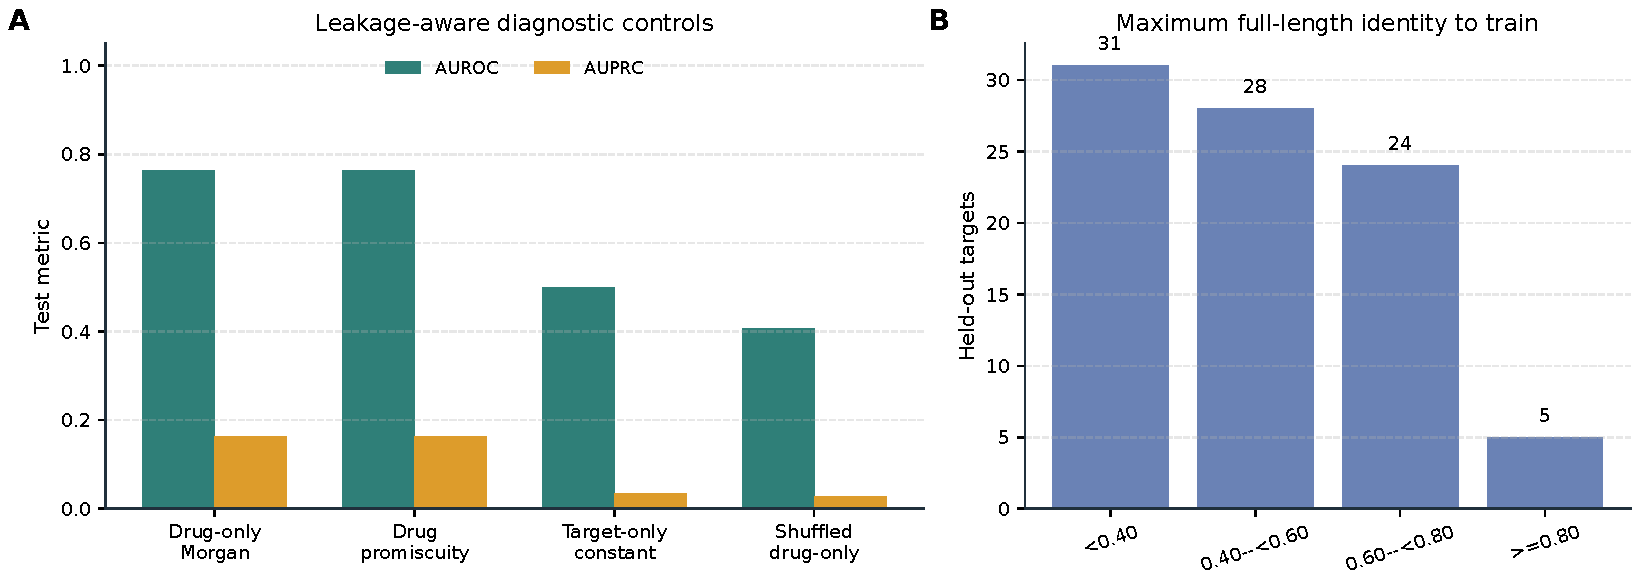
\includegraphics[width=\linewidth]{figures/fig_reviewer_controls.pdf}
\caption{\textbf{Diagnostic controls and target-relatedness audit.}
  Panel A: leakage-aware controls on the exact-sequence-grouped cold-target
  test. Drug-only and drug-promiscuity scores use no target
  representation; the target-only constant is the only target-only control that
  does not use held-out target labels.  Panel B: number of held-out targets by
  maximum full-length global sequence identity to any training target.}
\label{fig:diagnostic_controls}
\end{figure}

Under the Drug-ID-held-out split, BioInteract achieves AUROC~$=0.733$ in the canonical
current-release reconstruction. The fingerprint audit is included to clarify that Drug-ID-held-out means
unseen compound identifiers, not an externally validated scaffold-hopping or
out-of-distribution guarantee.

\subsection{Strict External BindingDB Evaluation}

We next performed the pre-specified, frozen external evaluation on the curated
BindingDB cohort.  After all measurement-quality, exact-identity novelty, and
replicate-consistency filters, it contains 1{,}932 pairs from 1{,}195 ligands
and 396 targets: 516 high-affinity and 1{,}416 low-affinity pairs
(Table~\ref{tab:bindingdb_external}).  The model was neither retrained nor
recalibrated, and no BindingDB label was used to choose the checkpoint or
threshold.

The frozen checkpoint achieved AUROC $=0.560$ (95\% CI 0.531--0.589) and
AUPRC $=0.340$ (95\% CI 0.314--0.372).  At the frozen Davis threshold, F1 was
0.070, precision was 0.731, and recall was 0.037.  Thus, although the exact
double-novel cohort is a valid external test, it does not support a broad DTI-transfer claim.
Instead, it shows limited transfer from this
Davis-trained classifier to the broader BindingDB cohort.  This external result
does not alter the within-Davis checkpoint reconstructions and is not used to
interpret attention, residue attribution, binding pockets, or mechanisms.

\begin{table}[htbp]
\centering
\caption{Frozen strict external evaluation on BindingDB\cite{gilson2016bindingdb}.
The source uses exact $K_d$ measurements only; ligand and full protein-sequence
overlap with all Davis records were excluded.  AUROC and AUPRC intervals are
600-replicate pair-stratified bootstrap 95\% confidence intervals.}
\label{tab:bindingdb_external}
\begin{tabular}{lrrrr}
\toprule
\textbf{Cohort} & \textbf{Pairs / positives} & \textbf{AUROC} & \textbf{AUPRC} & \textbf{F1} \\
\midrule
BindingDB, strict double-novel & 1{,}932 / 516 & 0.560 [0.531, 0.589] & 0.340 [0.314, 0.372] & 0.070 \\
\bottomrule
\end{tabular}
\end{table}

\subsection{Training Dynamics}

Fig.~\ref{fig:training} reports a single checkpoint-matched, contiguous
validation-AUROC and training-loss trace for each archived protocol. The
duplicated Random trace and two restarted Target-ID fragments were excluded
because their epoch counters reset or their peak validation AUROC did not match
the released checkpoint. These plots describe observed optimisation paths only;
they do not establish absence of overfitting, quantify validation-loss behaviour,
or estimate repeated-seed variability.

\begin{figure}[htbp]
\centering
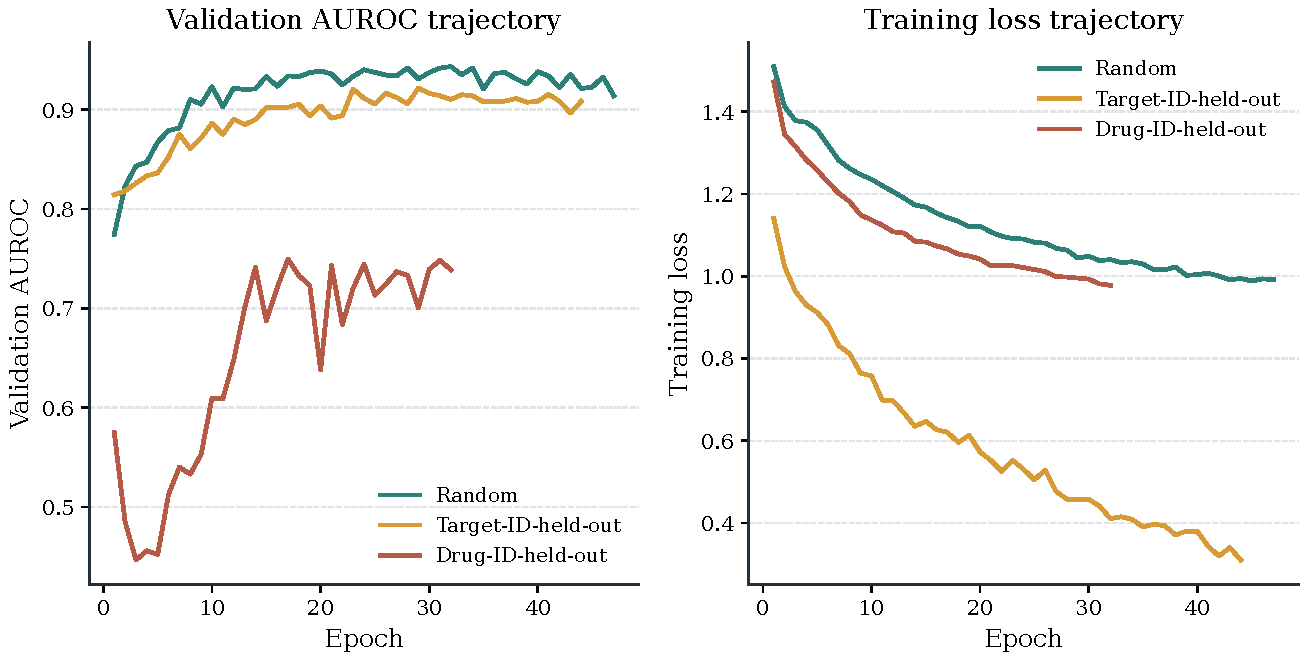
\includegraphics[width=\textwidth]{figures/fig4_training.pdf}
\caption{\textbf{Training dynamics across splitting protocols.}
  Panel A: validation AUROC over training epochs.  Panel B: training loss curves.
  Each line is one contiguous archived trace whose peak validation AUROC agrees
  with the saved checkpoint; duplicated and restarted segments are not plotted.
  No fitted or interpolated trends are shown. The trajectories do not establish
  absence of overfitting, validation-loss behaviour, or repeated-seed variability.}
\label{fig:training}
\end{figure}

\FloatBarrier

\subsection{Interpretability: Cross-Attention Analysis}
\label{sec:interpretability}

All interpretability figures and tables are derived directly from the saved
case-level outputs in the project interpretability-results directory, including
the report JSON and the corresponding heatmap, profile, and Grad-CAM renderings.
Accordingly, we report the model's actual residue-level attention and atom-level
Grad-CAM outputs rather than schematic placeholders.  These are attribution
outputs of the trained model, not independently validated residue contacts or
functional-group assignments.

\subsubsection{Global Attention Sparsity}

Analysis of cross-attention patterns across all 1{,}506 positive Davis
drug--target pairs
reveals a global attention sparsity of \SI{99.2}{\percent}
(Table~\ref{tab:global_attn}, Fig.~\ref{fig:sparsity}) under the stated
normalisation threshold. Figure~\ref{fig:sparsity} is computed directly from
the archived 1{,}301{,}380 pair-normalised residue scores, not from summary
bars; its top 1\% and 5\% of scores account for 78.9\% and 90.4\% of their
total attribution mass, respectively. This describes concentration of model
attribution; it does not demonstrate the size or location of a physical binding
interface.

\begin{table}[htbp]
\centering
\caption{Global cross-attention statistics computed across all 1{,}506 positive
  Davis pairs using \texttt{checkpoints/best.pt}. The values quantify the
  concentration of the model's pair-normalised
  residue-attribution scores; they do not provide structural validation of a
  binding pocket.}
\label{tab:global_attn}
\begin{tabular}{p{0.72\linewidth}c}
\toprule
\textbf{Metric} & \textbf{Value} \\
\midrule
Mean residue attention      & 0.0044 \\
Median residue attention    & 0.0003 \\
Top-1\% threshold           & 0.0572 \\
Top-5\% threshold           & 0.0036 \\
Fraction of residues with normalised attribution $<0.1$ of the pair-specific maximum & 99.2\% \\
Top 1\% / top 5\% cumulative attribution mass & 78.9\% / 90.4\% \\
Samples analysed            & 1{,}506 \\
Residue-score observations   & 1{,}301{,}380 \\
\bottomrule
\end{tabular}
\end{table}

\begin{figure}[htbp]
\centering
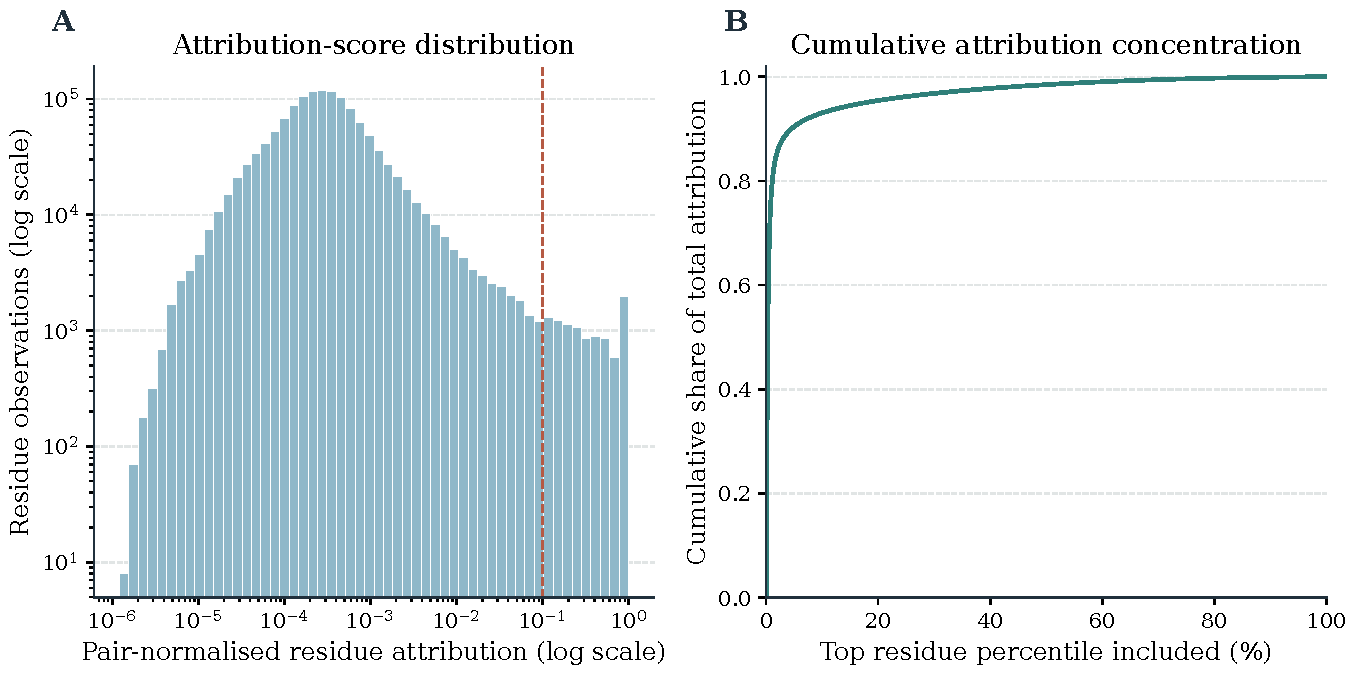
\includegraphics[width=\linewidth]{figures/fig5_attention_sparsity.pdf}
\caption{\textbf{Attention sparsity analysis.}
  (A)~Histogram of the archived pair-normalised per-residue attention scores
  across all 1{,}506 positive Davis pairs (1{,}301{,}380 observations; logarithmic
  axes); the dashed line denotes the 0.1 sparsity threshold. (B)~Cumulative
  attribution mass after sorting those same scores in descending order. The
  \SI{99.2}{\percent} value is an attribution-concentration statistic, not a
  claim about a contiguous protein-surface region.}
\label{fig:sparsity}
\end{figure}

\FloatBarrier

Although softmax attention is dense before normalisation, the observed
concentration arises after training on the limited and imbalanced Davis data.
It may reflect learned regularities, data composition, or both; it is therefore
not presented as independent evidence that the model has recovered molecular
recognition principles.

\subsubsection{Audit of Nominal ABL1 Variant Inputs}

A post-hoc audit of the exact Davis model inputs identified 15 target records
whose nominal names begin with ABL1, including the wild-type and the named
F317I, F317L, M351T, and E255K records.  All 15 records have the same
1,167-residue amino-acid sequence and SHA-256 digest in
\texttt{target\_sequences.csv} (Supporting Information, Table~S9).
Several nominal ABL1 variant identifiers in the Davis records used here are
associated with identical amino-acid sequences. Consequently, the present model
inputs do not encode the corresponding mutation-specific sequence changes, and
BioInteract cannot be evaluated for mutation-specific or resistance-specific
behaviour using these records. We therefore withdraw the previous
mutant-comparison analysis and draw no resistance-related conclusion.

\subsection{Case Study: Functional-Group Attribution}

The saved Grad-CAM output for the non-mutant EGFR--D0014 Davis pair provides a
compact example of atom-level scores aggregated to functional groups
(Table~\ref{tab:functional_group}).  The entries are model-native attribution
scores rather than measured contacts or interaction types.

\begin{table}[htbp]
\centering
\caption{Model-native functional-group attribution for the archived EGFR--D0014
  Davis case. Scores are normalised atom-level Grad-CAM values aggregated by
  functional group; they do not identify physical contacts.}
\label{tab:functional_group}
\begin{tabular}{lc}
\toprule
\textbf{Functional Group} & \textbf{Importance} \\
\midrule
Carbonyl       & 0.431 \\
Amide          & 0.389 \\
Ether          & 0.136 \\
Halogen        & 0.134 \\
Amino          & 0.090 \\
Aromatic ring  & 0.000 \\
Heterocyclic N & 0.000 \\
\bottomrule
\end{tabular}
\end{table}

\subsection{Cross-Case Functional-Group Attribution Variation}

The two non-mutant saved cases differ markedly in their classifier scores and
attribution profiles (Table~\ref{tab:functional_group_comparison}).  EGFR--D0014
has a high-affinity-class score of 0.995 and its largest aggregated groups are
carbonyl (0.431) and amide (0.389).  BRAF--D0023 has a score of 0.099 and only
small saved values for aromatic ring (0.059) and hydroxyl (0.000), despite its
archived positive affinity of 0.19 nM. We therefore treat BRAF--D0023 as a
low-scoring failure-mode example for an experimentally positive pair. This is a
descriptive limitation of model behaviour, not an explanation of target binding
or an assessment of functional-group chemistry.

\begin{table}[htbp]
\centering
\caption{Cross-case model-native functional-group attribution. Classifier
  scores and group values are saved-output summaries for the non-mutant
  EGFR--D0014 and BRAF--D0023 Davis cases.}
\label{tab:functional_group_comparison}
\begin{tabular}{lccc}
\toprule
\textbf{Case} & \textbf{Class score} & \textbf{Largest group} & \textbf{Score} \\
\midrule
EGFR--D0014 & 0.995 & Carbonyl & 0.431 \\
BRAF--D0023 & 0.099 & Aromatic ring & 0.059 \\
\bottomrule
\end{tabular}
\end{table}

\FloatBarrier

%%====================================================================
\section{Discussion}
\label{sec:discussion}
%%====================================================================

\subsection{From Prediction Accuracy to Inspectable Hypotheses}

BioInteract is intended to make model behaviour more inspectable than a purely
scalar DTI prediction.  Its attention matrices and Grad-CAM scores can generate
hypotheses about which representations contributed to a prediction.  Such
hypotheses can subsequently be assessed with crystal structures, mutagenesis,
or structure--activity relationship (SAR) experiments; the present study does
not replace these measurements.

The contextual random-split comparison places the canonical BioInteract result
below the historical DrugBAN AUROC and above its historical AUPRC; because the
protocols and pretraining are unmatched, this is not a comparative performance
claim. These Davis results do not show that
BioInteract maps a physical binding pocket, assigns an interaction type to an
atom pair, ranks a large compound library, or assesses treatment resistance.

\subsection{The 99.2\% Attention Sparsity}

The observed \SI{99.2}{\percent} attention sparsity is a property of the
pair-normalised, residue-pooled attribution scores under the chosen threshold. Although it is
compatible with a model focusing on a small subset of residues, it can also be
affected by the kinase-focused and imbalanced training data.  It should not be
read as evidence that the highlighted residues constitute a true binding site.

\subsection{Scope of Cold-Start Evaluation}

The audit of the original Target-ID-held-out split identified exact duplicate
sequences across the training and test partitions. The newly added exact-sequence-grouped
cold-target and exact-sequence-grouped cold-both evaluations provide a stricter within-Davis stress
test, but they still involve kinase proteins and do not demonstrate performance
on unrelated protein families or pocket classes.

The Drug-ID-held-out result is likewise restricted to the chemical diversity of 68
kinase inhibitors.  The observed Morgan-similarity distribution documents the
nearest-neighbour relationship between held-out and training molecules, but it
does not establish scaffold hopping or out-of-distribution robustness.

\subsection{Diagnostic Controls and Remaining Dataset Bias}

The exact-sequence-grouped cold-target diagnostic controls demonstrate that a target-independent
drug representation retains substantial ranking signal in Davis.  The
drug-only Morgan and drug-promiscuity controls each achieve AUROC near 0.764,
whereas BioInteract reaches 0.873 under the same exact-sequence-grouped
partition.  This improvement is compatible with the use of target information,
but it neither excludes ligand-side activity bias nor establishes that the model
has learned a molecular-recognition mechanism.  We therefore interpret the
control comparison as a boundary on the Davis result, not as causal evidence for
any particular encoder or attribution map.  The label-shuffled control confirms
that the observed drug-only signal depends on the training labels; it is not a
test of structural interaction recovery.

\subsection{Functional-Group Attribution Without Structural Supervision}

The Grad-CAM functional-group ranking is qualitatively compared with kinase
SAR literature, but it remains a gradient-based attribution.  In particular,
the analysis does not determine whether a group forms a hydrogen bond, a
pi-stacking interaction, a cation--pi interaction, or a van der Waals contact,
nor whether an implicated protein residue contributes through its backbone or
side chain.  These questions require a structural complex or targeted
experiments.\cite{zhang2009targeting}

\subsection{Limitation of Nominal ABL1 Variant Records}

The exact-input audit shows that the nominal ABL1 variant labels do not supply
variant-specific sequence information to the present model. We therefore remove
the former mutant-comparison figures, tables, and conclusions. The Davis records
remain useful as labelled kinase interactions, but they cannot support an
analysis of mutation effects or drug resistance in this study.

\subsection{Future Directions}

The strict BindingDB evaluation directly indicates limited transfer beyond the
Davis benchmark; it therefore cannot support a protein-family-agnostic,
broad-pocket, or chemical-space generalisation claim.  Evaluation after
retraining and validation on a wider, pre-specified multi-family protocol is
required to establish whether the limitation arises from the Davis training
distribution, task definition, or model. Direct comparison with independent
experimental evidence is also needed before attributions can be assigned a
structural meaning.

No overlap analysis between the Davis cases and PDBBind or LP-PDBBind, and no
PLIP contact validation, was performed in this study. A future structural audit
should use a non-overlapping benchmark of experimentally resolved complexes,
predefine the atom--residue contact criterion, and compare model attributions
with the resulting contact labels (for example, from PLIP) before structural
meaning is assigned.\cite{salentin2015plip}

The present implementation was audited on one NVIDIA GPU. Although the
2{,}442{,}083 trainable parameters do not increase with the number of training
pairs, data-processing time, graph batching, ESM-2 embedding extraction and
storage, and accelerator memory must be profiled at larger scale. Distributed
training was not evaluated, and no claim is made that the current implementation
scales linearly to BindingDB-sized data.

Evaluation on curated allosteric and cryptic-site benchmarks, with appropriate
structural or dynamic context, is likewise required before BioInteract can be
assessed for non-canonical drug--target interactions.  Existing work highlights
the need for explicit allosteric-site labels and benchmark design,\cite{wu2022allostericbenchmark,gatlin2026allostericgrammar}
and for structural or dynamic treatment of cryptic pockets.\cite{zhang2026crypticpockets}
CryptoBench provides a dedicated cryptic protein--ligand benchmark that can help
define such a future evaluation.\cite{skrhak2024cryptobench}

Extending BioInteract from binary interaction classification to
continuous binding-affinity regression ($pK_d$) would provide the finer-grained
potency estimates needed for lead optimisation, where accurate ranking of closely
related analogues is as important as binary activity prediction.

%%====================================================================
\section{Conclusion}
\label{sec:conclusion}
%%====================================================================

We have presented BioInteract, a DTI-prediction framework that combines
chemistry-aware molecular graph encoding, ESM-2/physicochemical residue
representations, and bidirectional cross-attention.  The model provides
prediction scores together with inspectable model-native attention and Grad-CAM
attributions.

The revision clarifies the evidence boundary of these outputs.  The observed
attention concentration and functional-group ranking describe model behaviour;
neither is a validated three-dimensional mechanism or binding-contact prediction.
We also distinguish Target-ID-held-out performance
from exact-sequence-grouped cold-start evaluation after detecting duplicate
sequences in the original target partition.  Broader datasets and direct
structural validation remain necessary for generalisation and mechanistic claims.
In particular, the strict external BindingDB test shows limited transfer of the
frozen Davis checkpoint, rather than establishing broad DTI transfer.

BioInteract is available as a publicly accessible interactive web interface at
\url{https://huggingface.co/spaces/AI4deeperScience/BioInteract} for the
custom-prediction workflow shown in Fig.~\ref{fig:webserver}.  The repository
README documents the command-line workflow for the available attribution
outputs.

\begin{figure}[htbp]
  \centering
  \begin{minipage}[t]{0.34\linewidth}
    \textbf{A}\par\smallskip
    
\includegraphics[width=\linewidth]{figures/WEB.png}
  \end{minipage}\hfill
  \begin{minipage}[t]{0.63\linewidth}
    \textbf{B}\par\smallskip
    
\includegraphics[width=\linewidth,trim=130bp 50bp 420bp 1300bp,clip]{figures/WEB.png}
  \end{minipage}
  \caption{\textbf{BioInteract interactive web server.}
    Panel A shows the full screenshot of the publicly accessible interface at
    \url{https://huggingface.co/spaces/AI4deeperScience/BioInteract}.
    Panel B enlarges the attribution region from the same screenshot. The interface
    shows the custom-prediction input and prediction-result state
    for human Aurora kinase C (UniProt Q9UQB9).  It displays the entered SMILES,
    protein sequence, and high-affinity-class classifier score (sigmoid output).
    The enlarged lower portion displays the generated atom--residue attention
    map and the ``Top 10 Residue Attributions'' chart.  These are model-native
    attribution views, not physical-contact or hotspot labels.  Command-line
    instructions for generating the available attribution outputs are provided
    in the public repository.}
  \label{fig:webserver}
\end{figure}

BioInteract represents a step toward AI-assisted DTI prediction in which model
scores are accompanied by transparent attribution outputs and explicit limits on
their interpretation.  Such outputs are most useful when combined with rigorous
split auditing, external validation, and biochemical experiments.

%%====================================================================
\section*{Acknowledgements}
%%====================================================================

The authors thank Meta AI Research for providing the ESM-2 pretrained protein
language model and the RDKit developers for maintaining the open-source
cheminformatics toolkit.

%%====================================================================
\section*{Supporting Information}
%%====================================================================

The Supporting Information contains: model hyperparameters and feature details
(Tables~S1--S3); computational environment (Table~S4); dataset and split
statistics (Tables~S5--S7); atom features (Table~S8); the Davis ABL1
nominal-variant input audit (Table~S9); non-mutant EGFR and BRAF case summaries
(Tables~S10--S11); complete model parameter counts (Table~S12); and strict
BindingDB external-validation provenance and results (Table~S13).
This material is available free of charge.

%%====================================================================
\section*{Data Availability}
%%====================================================================

All data used in this study are publicly available. The Davis kinase inhibitor
dataset used for model training and evaluation is available from the original
publication.\cite{davis2011comprehensive} The external evaluation uses the official
BindingDB curated-articles TSV snapshot
\texttt{BindingDB\_BindingDB\_Articles\_202607}, obtained from the BindingDB
download service;\cite{gilson2016bindingdb} the raw archive remains available from
its source, and the release provides the deterministic curation and frozen
evaluation scripts plus manifest hashes. The immutable release containing the
released checkpoints, canonical prediction CSVs, provenance hashes, strict-split
artifacts, and reproduction scripts is archived at Zenodo,
\url{https://doi.org/10.5281/zenodo.21437753}. The BioInteract source repository
is hosted on \href{https://github.com/Liubo-520/bio-intelligence}{GitHub}. An interactive web
server for the custom-prediction workflow is available through the
\href{https://huggingface.co/spaces/AI4deeperScience/BioInteract}{BioInteract Space}; the README
documents the command-line attribution workflow.

\section*{Code Availability}

The BioInteract source code, pretrained model weights, configuration files,
canonical metric-reconstruction scripts, and figure-generation scripts are
publicly available through \href{https://github.com/Liubo-520/bio-intelligence}{GitHub} and
as the immutable Zenodo release, \url{https://doi.org/10.5281/zenodo.21437753}.
The interactive web
application for the custom-prediction workflow is available through the
\href{https://huggingface.co/spaces/AI4deeperScience/BioInteract}{BioInteract Space}.

%%====================================================================
\section*{Author Contributions}
%%====================================================================

\textbf{Shengnan Wang}: Conceptualisation, Methodology, Software, Formal
analysis, Writing -- original draft. \\
\textbf{Qi Zhang}: Methodology, Validation, Data curation, Visualisation,
Writing -- original draft. \\
\textbf{Xucheng Liu}: Investigation, Validation, Data curation. \\
\textbf{Zixuan Wang}: Software, Investigation, Data curation. \\
\textbf{Jiangke Cheng}: Resources, Validation, Visualisation. \\
\textbf{Zhi Huang}: Supervision, Writing -- review \& editing, Funding
acquisition, Corresponding author.

\vspace{0.5em}
\noindent S.\,Wang and Q.\,Zhang contributed equally to this work.
%%====================================================================

% Author A: Conceptualisation, Methodology, Software, Formal analysis, Writing -- original draft. \\
% Author B: Methodology, Validation, Data curation, Visualisation, Writing -- original draft. \\
% Author C: Investigation, Validation, Data curation. \\
% Author D: Software, Investigation, Data curation. \\
% Author E: Resources, Validation, Visualisation. \\
% Author F: Supervision, Writing -- review \& editing, Funding acquisition.

% \vspace{0.5em}
% \noindent Author A and Author B contributed equally to this work.
%%====================================================================
\section*{Declaration of Competing Interests}
%%====================================================================

The authors declare no competing interests.

\section*{Funding}

This work was supported by the Sichuan Provincial Key Laboratory for Development and Utilization of Characteristic Horticultural Biological Resources under Grant TSYY202502. The funder had no role in study design, data collection and analysis, decision to publish, or preparation of the manuscript.

\bibliography{references}
\end{document}
